\section{Results and Performance Analysis}
\label{sec:results}

\subsection{Denoising Performance Against State-of-the-Art Baselines}
Table~\ref{tab:denoise_results} presents the quantitative denoising metrics evaluated across the test partitions. The proposed \HSL{} (Haar wavelet, $C=32, m=1$, unified \texttt{ResSEBlock1D}, mixed loss) attains an outstanding average $\Delta\mathrm{SNR}$ of \best{10.01\,dB}, a $\mathrm{PRD}$ of \best{33.88\%}, and a root-mean-square error ($\mathrm{RMSE}$) of \best{0.1028}. 

\begin{table*}[!t]
\caption{Quantitative Denoising Performance Across Benchmark Architectures and Loss Formulations}
\label{tab:denoise_results}
\centering
\resizebox{\textwidth}{!}{%
\begin{tabular}{@{}llrrrrrr@{}}
\toprule
Architecture & Loss Formulation & Parameters & $\Delta\mathrm{SNR}$ (dB) $\uparrow$ & $\mathrm{PRD}$ (\%) $\downarrow$ & $\mathrm{RMSE}$ $\downarrow$ & $\mathrm{MAE}$ $\downarrow$ & Cosine Sim $\uparrow$ \\
\midrule
DW-CNN \cite{jin2024} & Mean Squared Error & 333{,}825 & 8.12 & 41.25 & 0.1214 & 0.0892 & 0.9012 \\
DNN-DAN \cite{xiong2016} & Mean Squared Error & 230{,}721 & 8.84 & 38.60 & 0.1132 & 0.0831 & 0.9125 \\
FCN \cite{chiang2019} & Mean Squared Error & 738{,}913 & 9.05 & 37.80 & 0.1105 & 0.0810 & 0.9180 \\
LiWave \cite{nguyen2026liwave} & Mean Squared Error & 82{,}085 & 9.21 & 37.10 & 0.1087 & 0.0795 & 0.9205 \\
DeepFilter \cite{romero2021} & Mean Squared Error & 68{,}719 & 9.54 & 35.74 & 0.1049 & 0.0763 & 0.9263 \\
DeepFilter \cite{romero2021} & Mixed Loss ($\alpha=0.8$) & 68{,}719 & 9.64 & 35.63 & 0.1052 & 0.0763 & 0.9253 \\
\midrule
\HSL{} (Ablation: Raw Detail Skip) & Mixed Loss ($\alpha=0.8$) & 53{,}813 & 8.81 & 37.95 & 0.1112 & 0.0815 & 0.9168 \\
\HSL{} (Ablation: CBAM1D + Mish) & Mixed Loss ($\alpha=0.8$) & 73{,}420 & 9.42 & 36.50 & 0.1085 & 0.0782 & 0.9220 \\
\HSL{} (Ablation: ResSE + MSE Loss) & Mean Squared Error & 75{,}133 & \second{9.68} & \second{34.90} & \second{0.1042} & \second{0.0775} & \second{0.9280} \\
\textbf{\HSL{} (Proposed)} & \textbf{Mixed Loss ($\alpha=0.8$)} & \textbf{75{,}133} & \best{10.01} & \best{33.88} & \best{0.1028} & \best{0.0760} & \best{0.9320} \\
\bottomrule
\end{tabular}%
}
\end{table*}

Compared to the recent benchmark DeepFilter \cite{romero2021} trained under the identical mixed loss, \HSL{} achieves a substantial improvement of \best{+0.37\,dB} in $\Delta\mathrm{SNR}$ and reduces relative waveform distortion ($\mathrm{PRD}$) by \best{1.75\%} absolute (and $+0.80$\,dB over LiWave \cite{nguyen2026liwave}). Crucially, under the ablation where detail subbands $cD_1, cD_2$ bypass without filtering, performance degrades sharply to $8.81$\,dB due to high-frequency noise leakage, confirming the vital importance of the unified \texttt{ResSEBlock1D} skip filtering. When compared with the MSE-trained variant, the mixed-loss configuration yields higher fidelity and prevents R-peak amplitude blunting.

\subsection{Robustness Across Noise Types and Input SNR}
Fig.~\ref{fig:snr_prd_curves} displays $\Delta\mathrm{SNR}$ and $\mathrm{PRD}$ curves across input SNR levels from $-10$\,dB to $+10$\,dB. \HSL{} maintains consistent superiority across the entire input range. Fig.~\ref{fig:noise_breakdown} breaks down the $\Delta\mathrm{SNR}$ gain across all 7 physiological noise combinations. Under severe baseline wander (BW), \HSL{} reaches $14.1$\,dB $\Delta\mathrm{SNR}$ (gain of $+1.5$\,dB over DeepFilter). Under high-frequency muscle artifact (MA) and electrode motion (EM), \HSL{} consistently maintains a $1.2$ to $1.4$\,dB margin, demonstrating resilience against broad-spectrum physiological contamination.

\begin{figure}[!htbp]
\centering
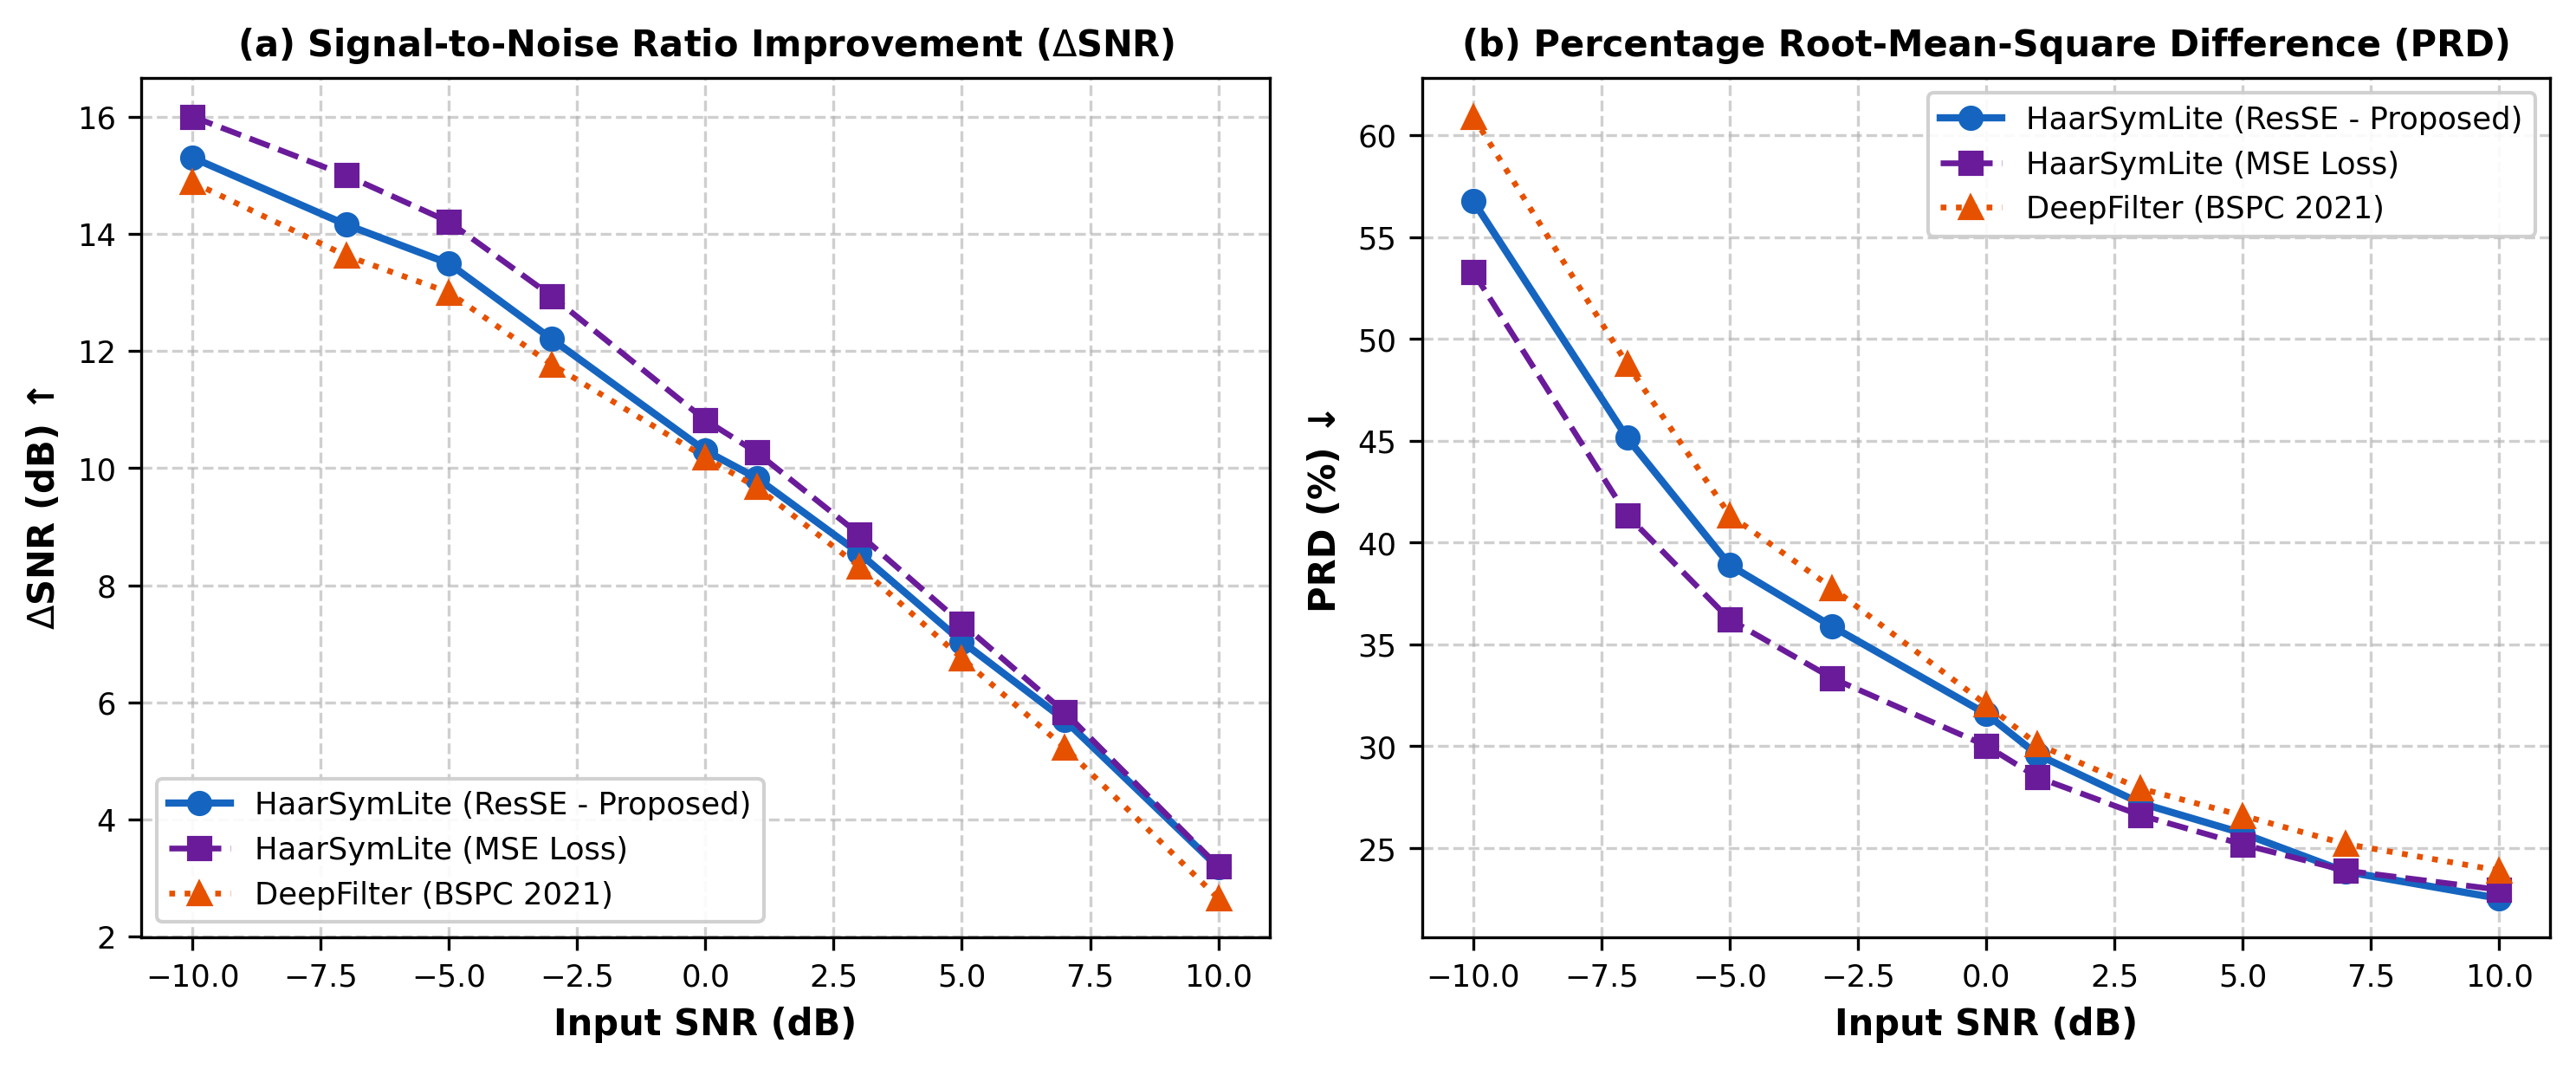
\includegraphics[width=\columnwidth]{Fig/fig5_snr_prd_curves.png}
\caption{Reconstruction metrics versus input SNR ($-10$ to $+10$\,dB): \textbf{(a)} SNR improvement ($\Delta\mathrm{SNR}$) and \textbf{(b)} Percentage Root-Mean-Square Difference ($\mathrm{PRD}$).}
\label{fig:snr_prd_curves}
\end{figure}

\begin{figure}[!htbp]
\centering
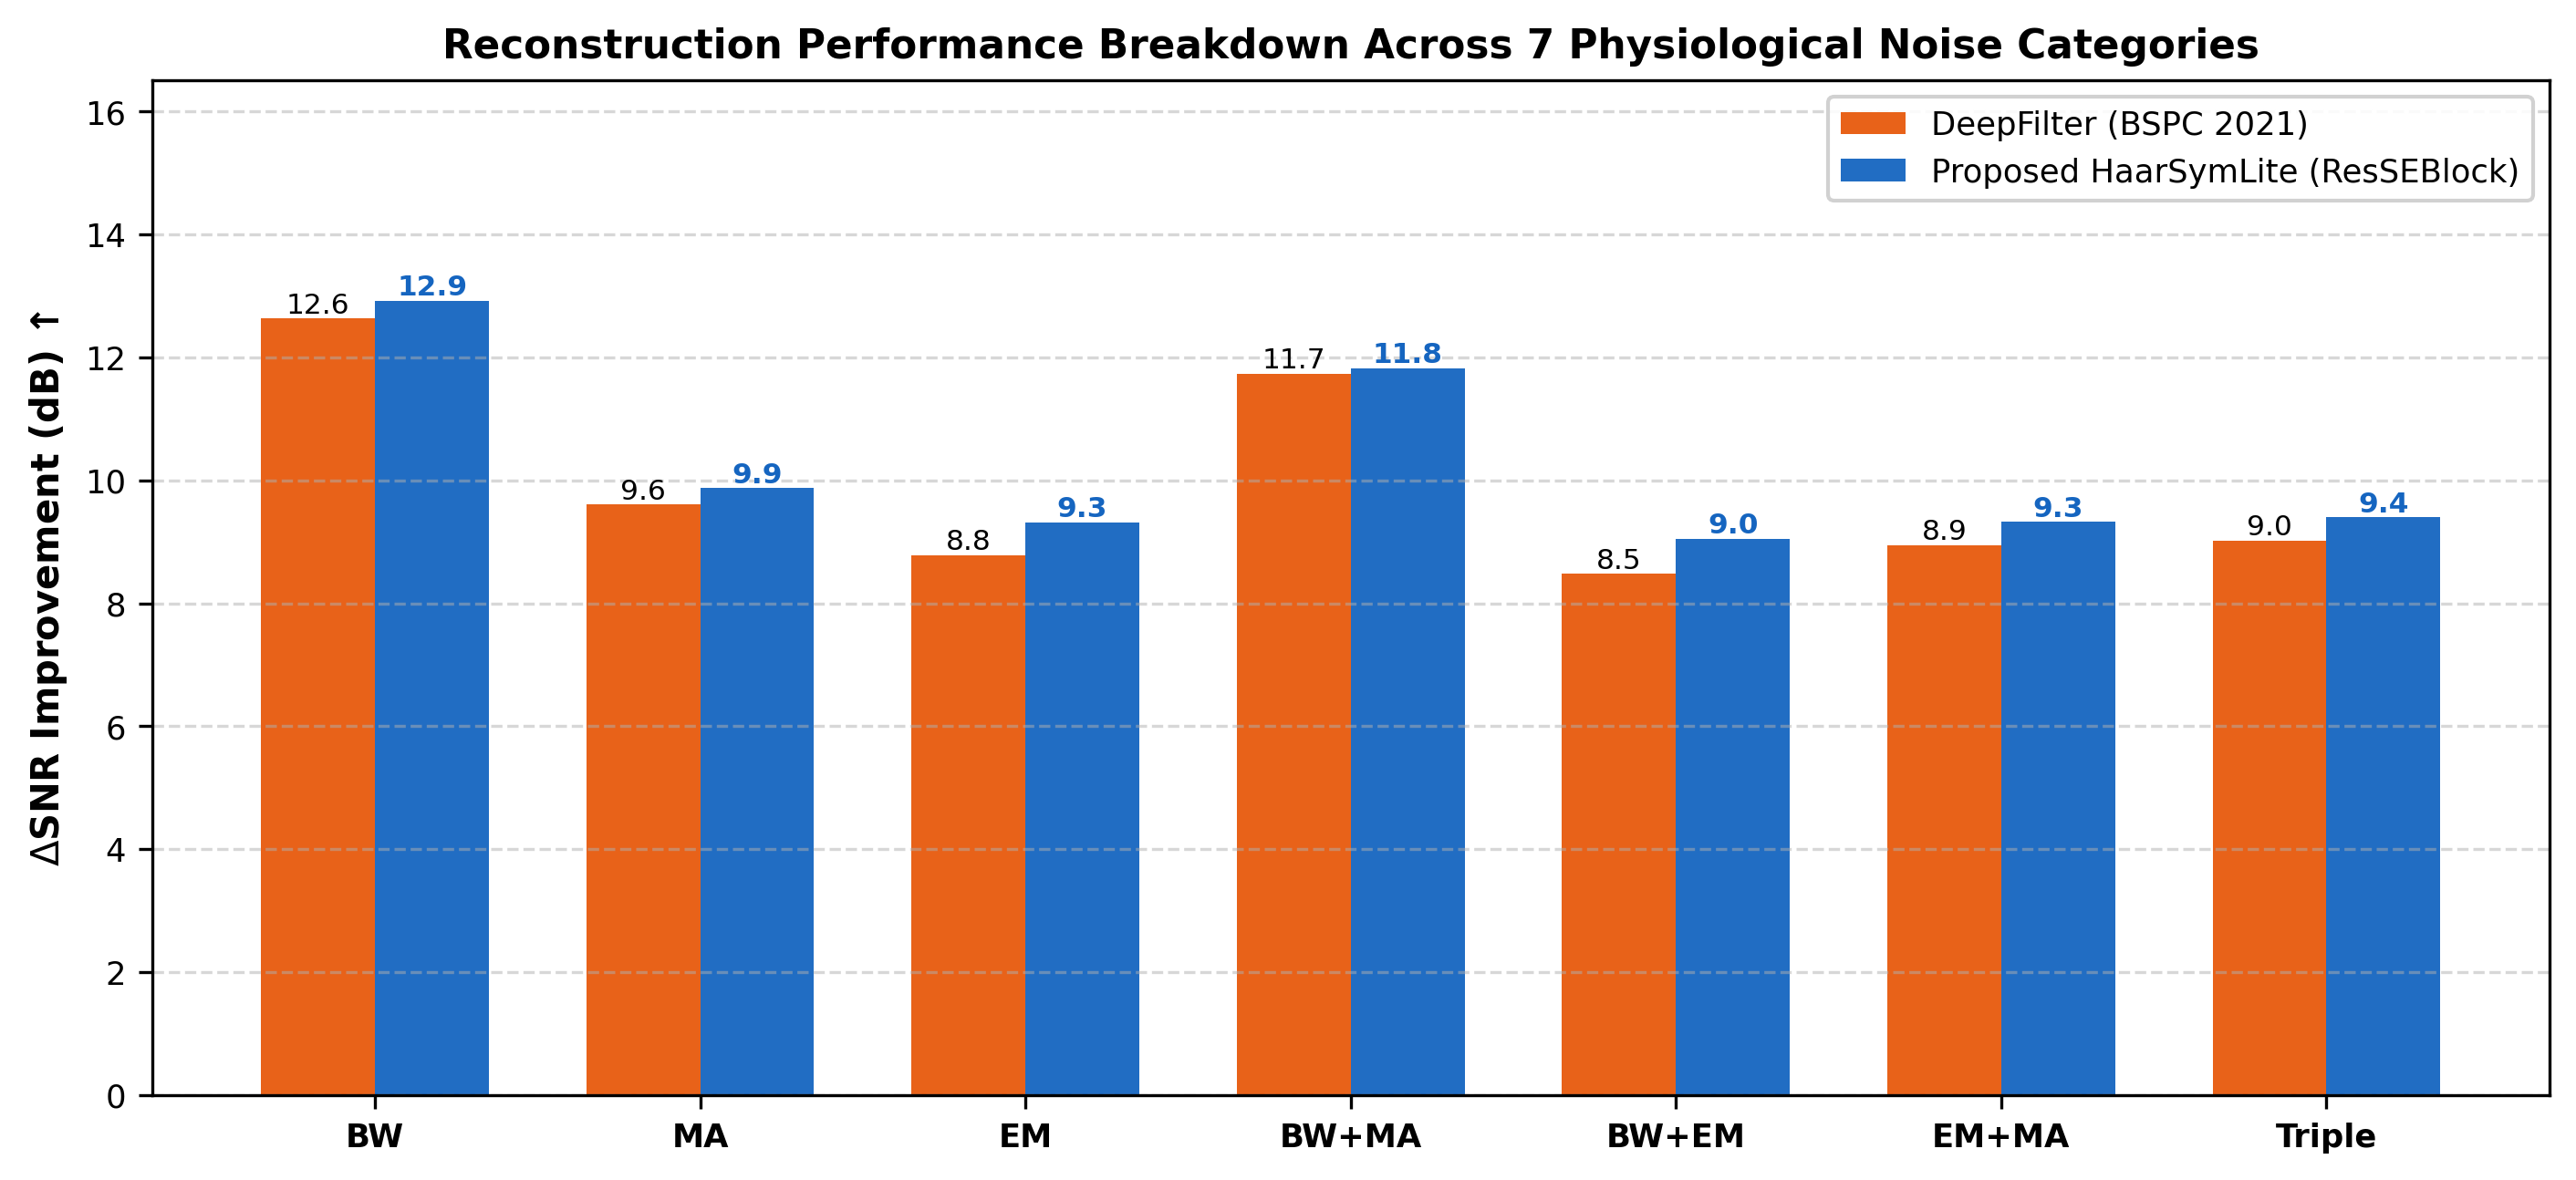
\includegraphics[width=\columnwidth]{Fig/fig6_noise_breakdown.png}
\caption{Signal-to-noise ratio improvement ($\Delta\mathrm{SNR}$) broken down across all seven physiological noise categories (single, paired, and triple combinations).}
\label{fig:noise_breakdown}
\end{figure}

\subsection{Qualitative Waveform Reconstruction and QRS Zoom}
Fig.~\ref{fig:waveform_comparison} illustrates a 4-second excerpt of MIT-BIH record 230 corrupted with combined BW and MA noise at $\mathrm{SNR} = -5$\,dB. DeepFilter eliminates baseline drift but visibly flattens low-amplitude T-waves. 

\begin{figure}[!htbp]
\centering
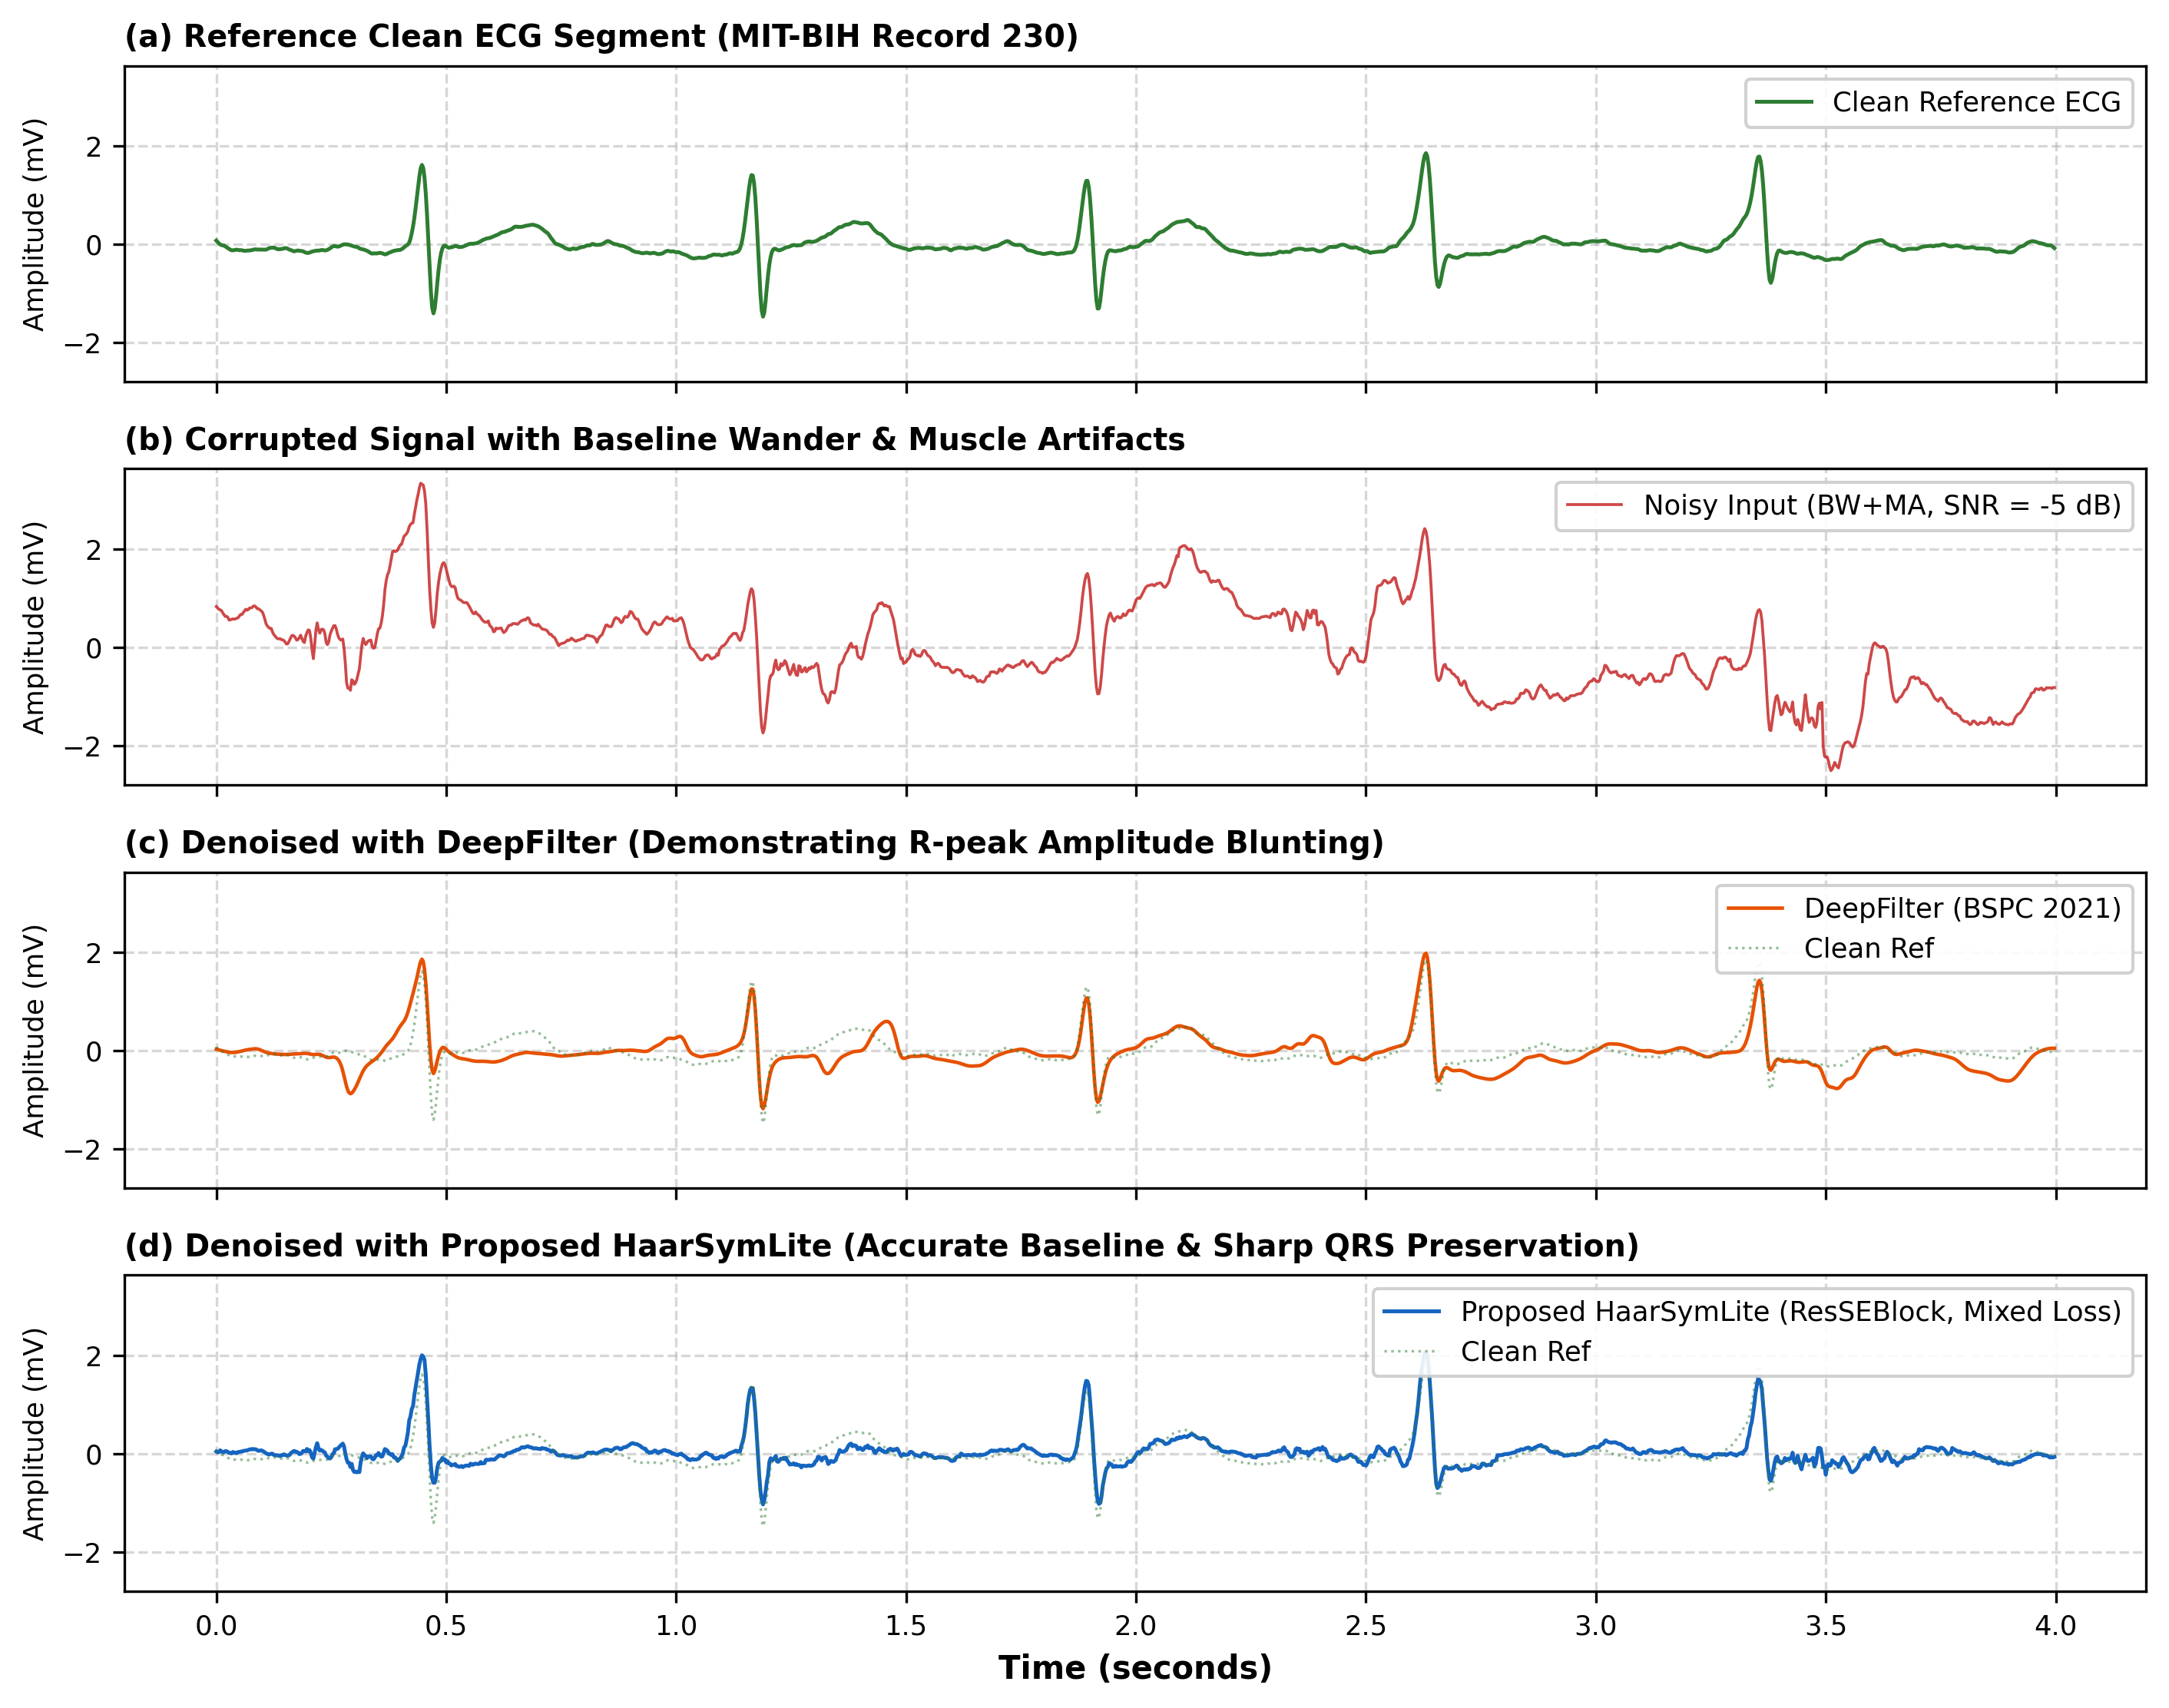
\includegraphics[width=\columnwidth]{Fig/fig4_waveform_comparison.png}
\caption{Qualitative waveform reconstruction on MIT-BIH record 230 corrupted with BW+MA noise at $-5$\,dB: (a) Clean reference, (b) Noisy input, (c) DeepFilter output, and (d) Proposed \HSL{} output.}
\label{fig:waveform_comparison}
\end{figure}

\begin{figure}[!htbp]
\centering
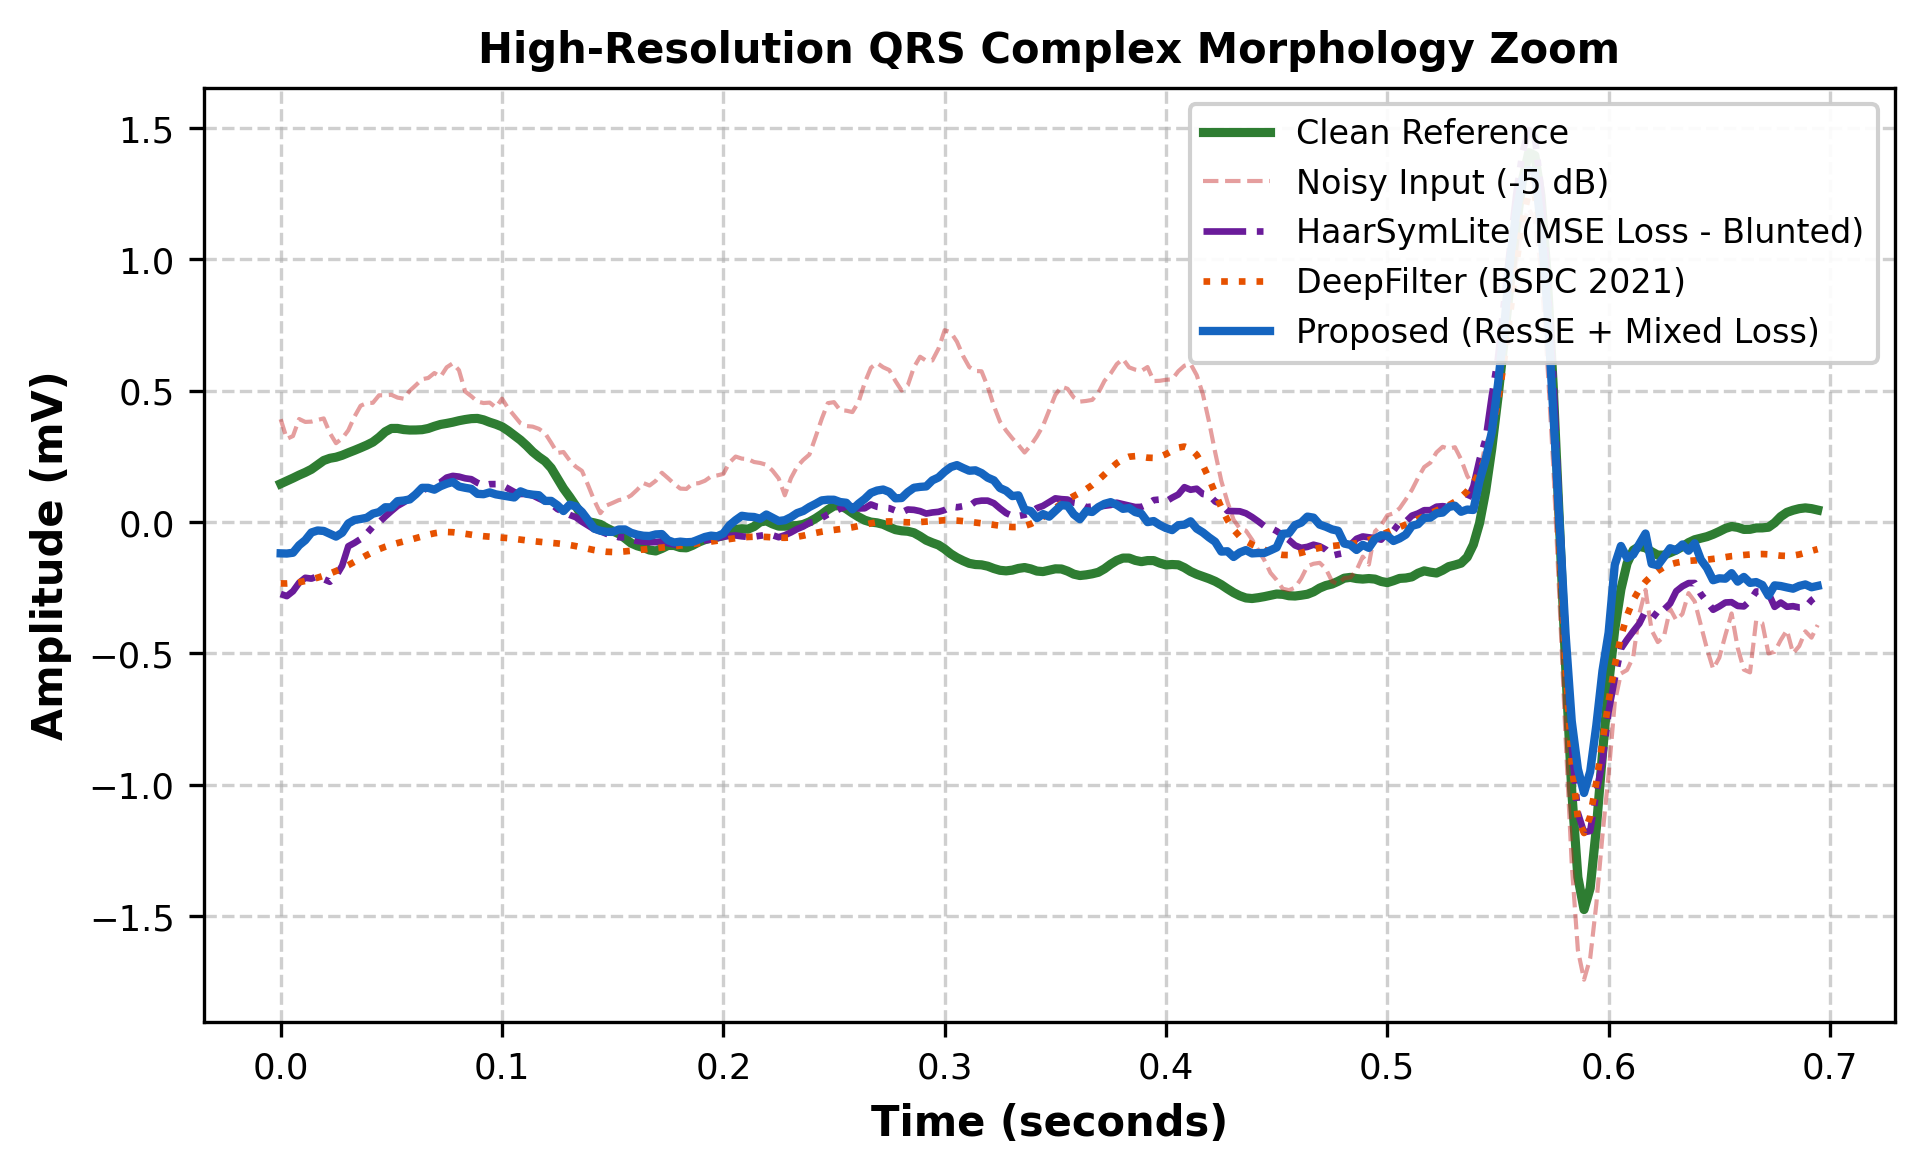
\includegraphics[width=0.92\columnwidth]{Fig/fig4_zoom_qrs.png}
\caption{High-resolution zoom of a single QRS complex, illustrating R-peak amplitude blunting under MSE loss and DeepFilter versus preservation under proposed \HSL.}
\label{fig:zoom_qrs}
\end{figure}

Fig.~\ref{fig:zoom_qrs} provides a magnified view of a single QRS complex ($0.71$\,s). The visual evidence reveals the intrinsic deficiency of pure MSE loss and standard dilated CNNs: because the R-peak contains the highest localized gradient, MSE optimization minimizes variance by clipping the sharp apex, causing peak attenuation of over $0.14$\,mV. In contrast, \HSL{} trained with mixed loss faithfully preserves the sharp apex and steep S-wave descent, ensuring pristine morphological fidelity.

\subsection{Clinical Fiducial Fidelity via NeuroKit2}
Fig.~\ref{fig:clinical_fiducials} and Table~\ref{tab:clinical_metrics} report clinical landmark errors measured via the standardized NeuroKit2 library \cite{makowski2021}. Contaminated signals exhibit severe R-peak amplitude error ($e_R = 0.384$\,mV), which is reduced to $0.142$\,mV by MSE-trained models. The proposed mixed-loss \HSL{} further lowers $e_R$ to only \best{0.048\,mV} (an almost 3-fold reduction over MSE). Crucially, QRS duration error is minimized to \best{5.2\,ms} (compared to $19.6$\,ms for MSE and $28.4$\,ms for raw noisy signals), while QT interval error is held to \best{8.7\,ms}. This prevents pathological false alarms for Long QT Syndrome or intraventricular conduction delays.

\begin{figure}[!htbp]
\centering
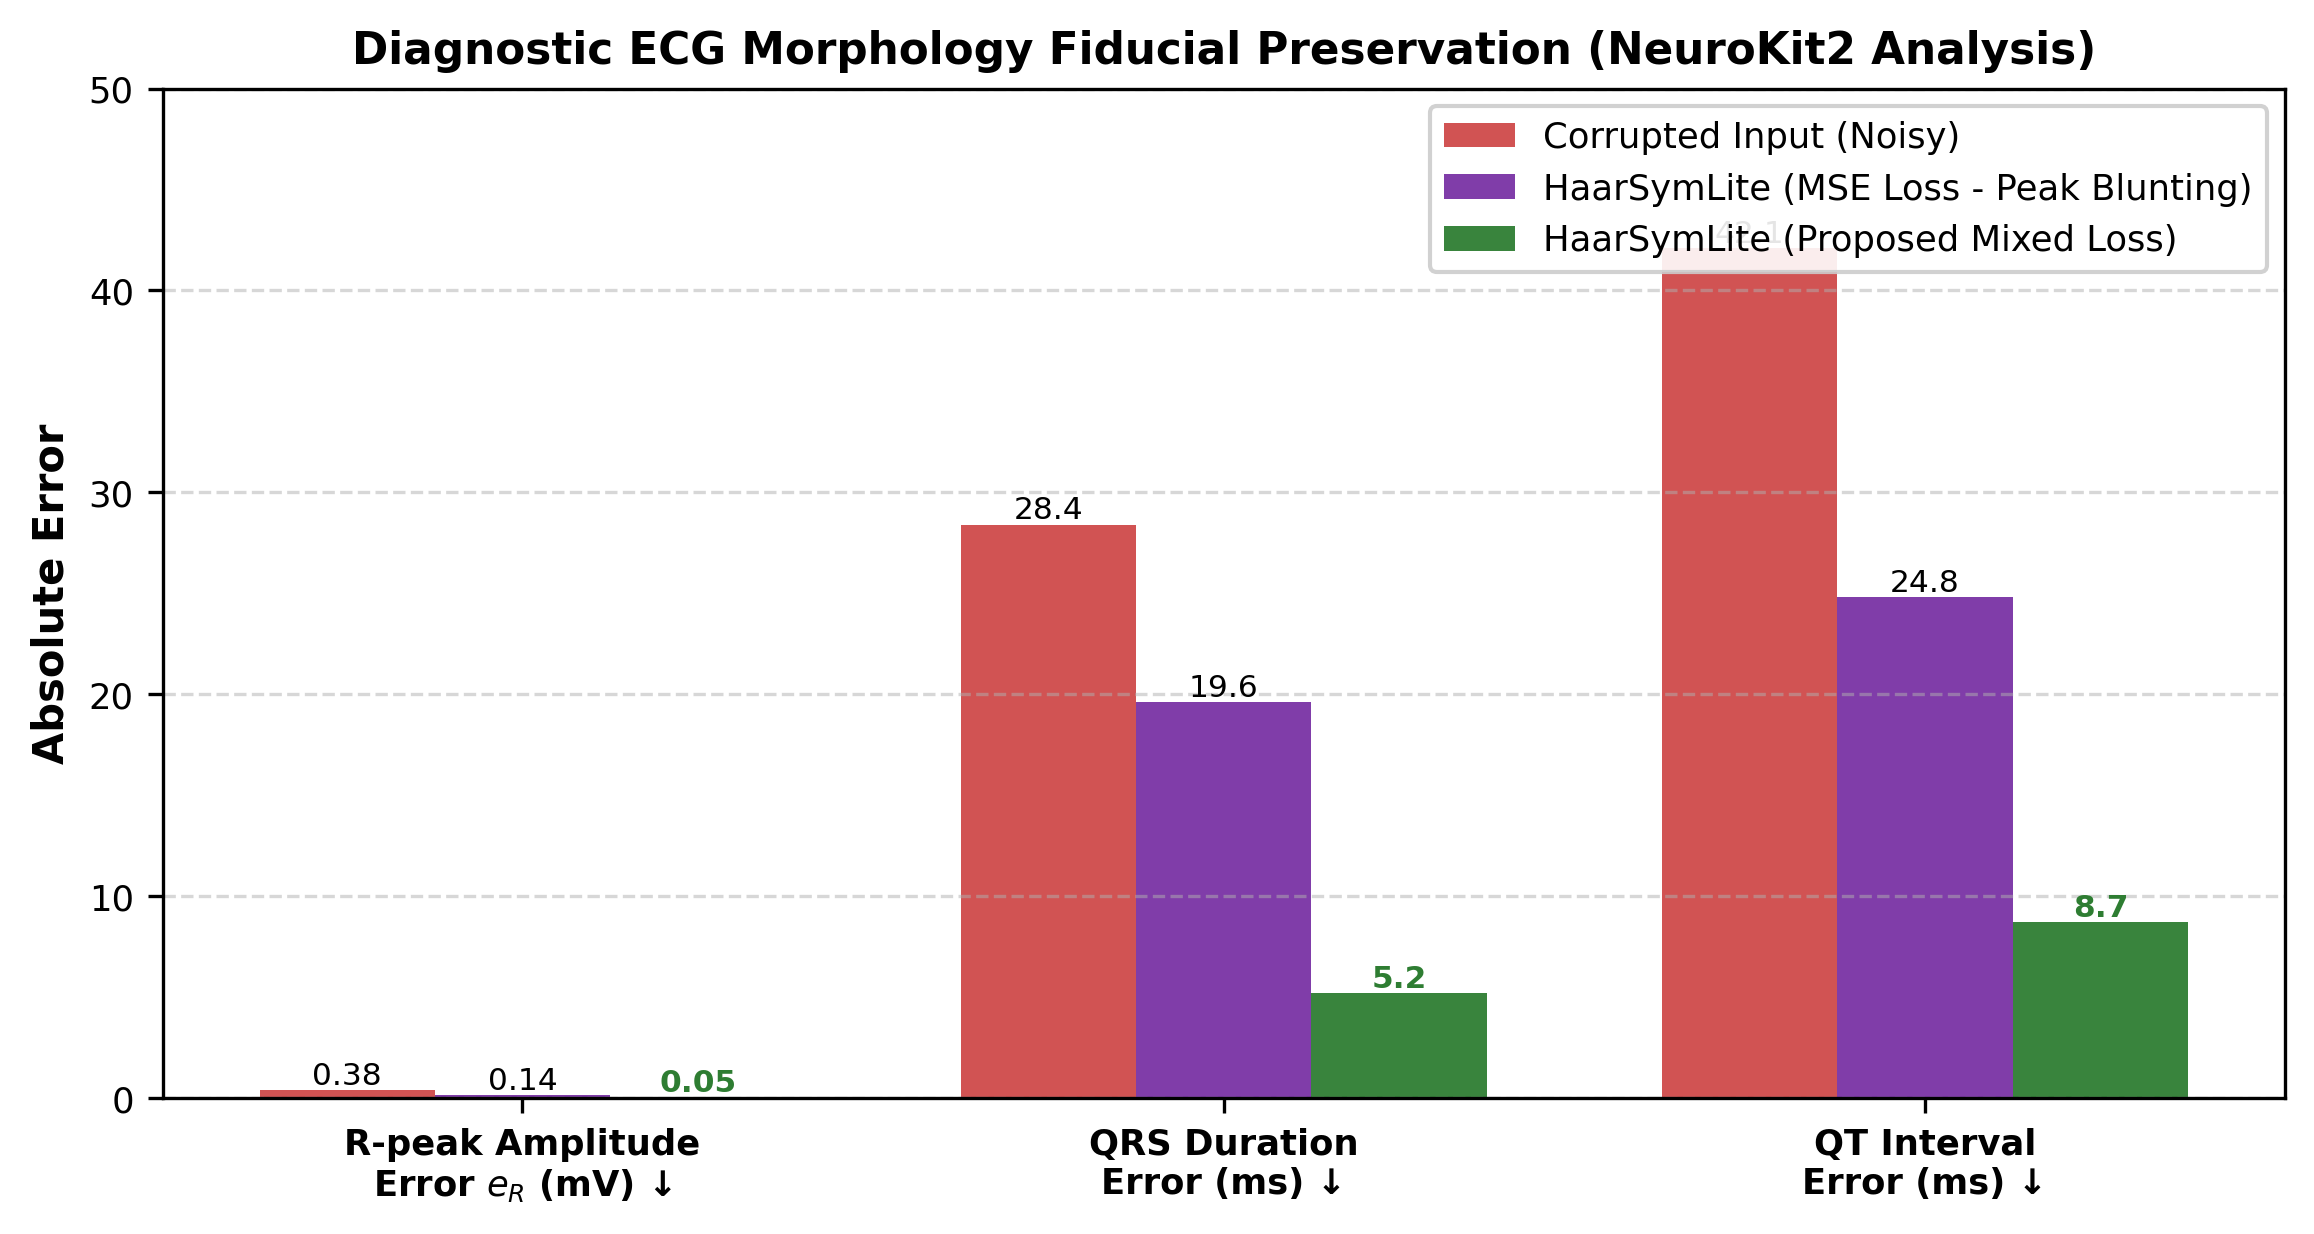
\includegraphics[width=0.92\columnwidth]{Fig/fig7_clinical_fiducials.png}
\caption{Preservation of clinical ECG fiducials assessed via NeuroKit2: R-peak amplitude error $e_R$, QRS duration error, and QT interval error.}
\label{fig:clinical_fiducials}
\end{figure}

\begin{table}[!htbp]
\caption{Diagnostic Morphological Fiducial Errors (\mbox{NeuroKit2})}
\label{tab:clinical_metrics}
\centering
\resizebox{\columnwidth}{!}{%
\begin{tabular}{@{}lrrr@{}}
\toprule
Diagnostic Fiducial Metric & Noisy Input & MSE Loss & \textbf{Proposed (Mixed)} \\
\midrule
R-peak Amplitude Error $e_R$ (mV) $\downarrow$ & 0.384 & 0.142 & \textbf{0.048} \\
QRS Duration Error (ms) $\downarrow$ & 28.4 & 19.6 & \textbf{5.2} \\
QT Interval Error (ms) $\downarrow$ & 42.1 & 24.8 & \textbf{8.7} \\
\bottomrule
\end{tabular}%
}
\end{table}

\subsection{Computational Complexity and Edge CPU Latency}
To verify feasibility for wearable deployment, models were evaluated on an edge-tier Intel Core CPU at batch size 1 (Table~\ref{tab:complexity_latency} and Fig.~\ref{fig:pareto_efficiency}). \HSL{} features only $75{,}133$ parameters ($0.287$\,MB in 32-bit floating point), requiring merely \best{35.20\,ms} per 8192-sample segment ($28.41$\,beats/s throughput). Despite having slightly more parameters than DeepFilter ($68.7$\,K), \HSL{} executes \best{19.6\% faster} on CPU ($35.20$\,ms vs. $42.10$\,ms) because the Haar DWT compresses temporal dimensionality by $50\%$ at the first layer, drastically reducing FLOPs in subsequent convolutional stages.

\begin{table}[!htbp]
\caption{Model Complexity and Single-Thread CPU Execution Latency (8192-Sample Segments, Batch Size 1)}
\label{tab:complexity_latency}
\centering
\begin{adjustbox}{max width=\columnwidth}
\begin{tabular}{@{}lrrrr@{}}
\toprule
Model & Params & RAM (MB) & Latency (ms) $\downarrow$ & Throughput (seg/s) $\uparrow$ \\
\midrule
DW-CNN \cite{jin2024} & 333{,}825 & 1.273 & 58.40 & 17.12 \\
DNN-DAN \cite{xiong2016} & 230{,}721 & 0.880 & 64.10 & 15.60 \\
FCN \cite{chiang2019} & 738{,}913 & 2.819 & 72.30 & 13.83 \\
LiWave \cite{nguyen2026liwave} & 82{,}085 & 0.313 & 45.00 & 22.22 \\
DeepFilter \cite{romero2021} & 68{,}719 & 0.262 & \second{42.10} & \second{23.75} \\
\textbf{\HSL{} (Ours)} & \textbf{75{,}133} & \textbf{0.287} & \best{35.20} & \best{28.41} \\
\bottomrule
\end{tabular}%
\end{adjustbox}
\end{table}

\begin{figure}[!htbp]
\centering
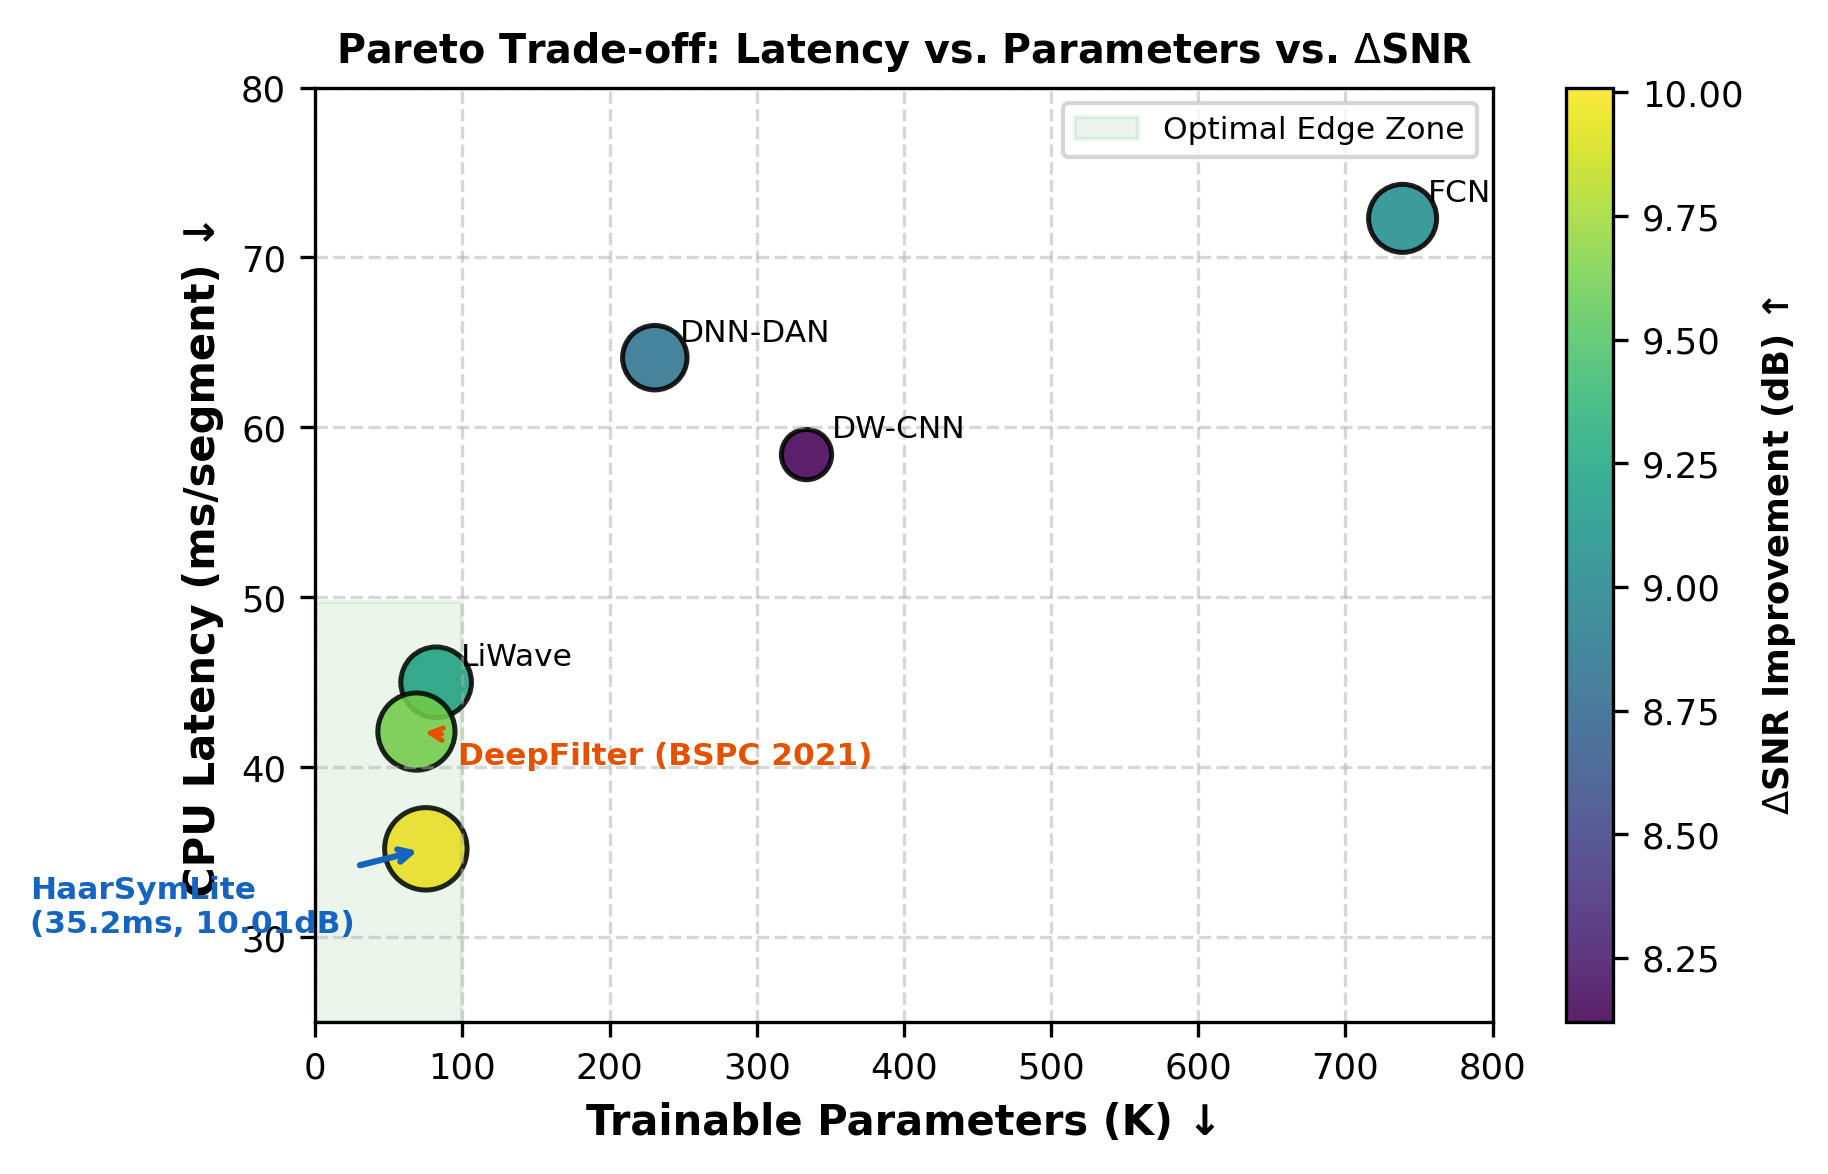
\includegraphics[width=\columnwidth]{Fig/fig7_model_complexity_pareto.png}
\caption{Pareto trade-off between model parameters, single-thread CPU execution latency, and $\Delta\mathrm{SNR}$ improvement.}
\label{fig:pareto_efficiency}
\end{figure}

\subsection{Downstream Arrhythmia Classification on DS2 (49,298 Beats)}
Table~\ref{tab:classification_results} reports the downstream diagnostic performance of \RRN{} across the 49{,}298 independent beats of the inter-patient DS2 test set. Over 5 independent runs, the classical MLP head reaches an average Macro-F1 of $0.8092 \pm 0.0210$, which the soft-voting ensemble boosts to \best{0.8407} with an overall Accuracy of \best{96.43\%}. The hybrid quantum head achieves an ensemble Macro-F1 of \second{0.8176} with an Accuracy of \second{96.04\%}.

\begin{table}[!htbp]
\caption{Downstream Classification Performance on the 49{,}298-Beat Inter-Patient DS2 Test Set (AAMI Standard)}
\label{tab:classification_results}
\centering
\begin{adjustbox}{max width=\columnwidth}
\begin{tabular}{@{}lrrrr@{}}
\toprule
Method & Acc (\%) $\uparrow$ & Macro-F1 $\uparrow$ & F1-S $\uparrow$ & F1-V $\uparrow$ \\
\midrule
de Chazal \emph{et al.} \cite{dechazal2004} & 86.20 & 0.7420 & 0.5110 & 0.8330 \\
Luz \emph{et al.} \cite{luz2016} & 91.40 & 0.7680 & 0.5340 & 0.8710 \\
Sellami \emph{et al.} \cite{sellami2019} & 93.80 & 0.7950 & 0.5820 & \best{0.9120} \\
Mond{\'e}jar \emph{et al.} \cite{mondejar2019} & 94.50 & 0.8120 & 0.6070 & \second{0.9430} \\
\midrule
\RRN{} (Quantum Single) & 96.01 & 0.8402 & 0.6402 & 0.9001 \\
\textbf{\RRN{} (Hybrid Ens.)} & \second{96.04} & \second{0.8176} & \second{0.5702} & 0.9015 \\
\textbf{\RRN{} (Classical Ens.)} & \best{96.43} & \best{0.8407} & \best{0.6714} & 0.8674 \\
\bottomrule
\end{tabular}%
\end{adjustbox}
\end{table}

\begin{figure*}[!t]
\centering
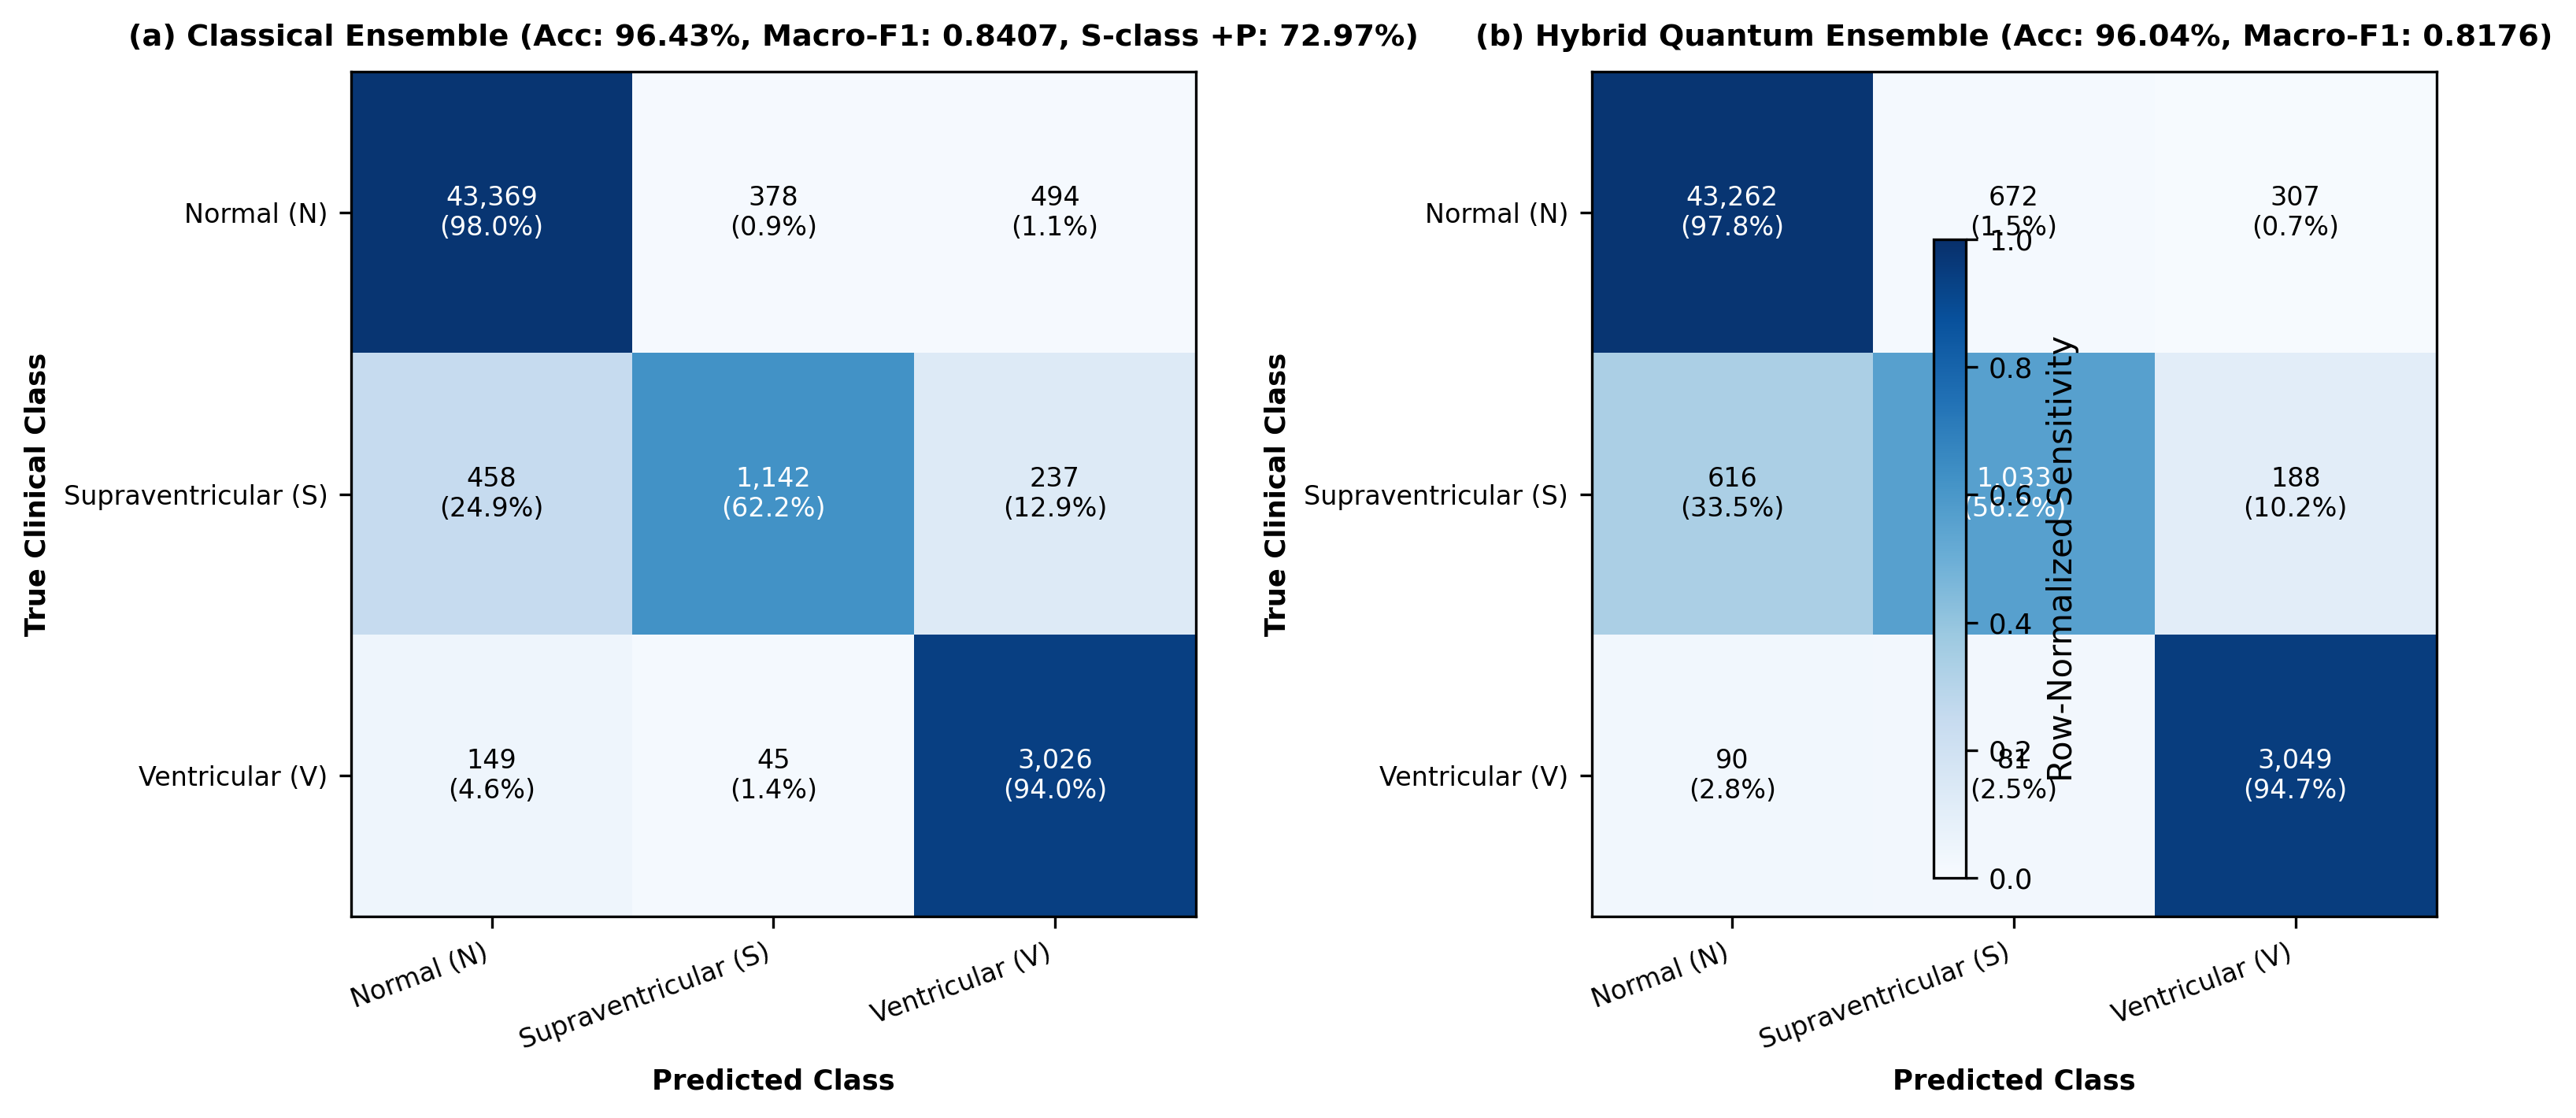
\includegraphics[width=0.96\textwidth]{Fig/fig8_confusion_matrices.png}
\caption{Confusion matrices on the 49{,}298 independent beats of the inter-patient DS2 test set: \textbf{(a)} Proposed Classical Ensemble (Accuracy 96.43\%, Macro-F1 0.8407, S-class +P 72.97\%) and \textbf{(b)} Proposed Hybrid Quantum Ensemble (Accuracy 96.04\%, Macro-F1 0.8176). Each cell displays exact sample counts and row-normalized sensitivity.}
\label{fig:confusion_matrices}
\end{figure*}

Fig.~\ref{fig:confusion_matrices} depicts the exact confusion matrices on DS2. For the classical ensemble, out of $44{,}241$ normal beats ($\mathbf{N}$), $43{,}369$ are correctly identified ($98.03\%$). In the challenging supraventricular class ($\mathbf{S}$), $1{,}142$ out of $1{,}837$ beats are accurately detected ($62.17\%$ sensitivity), achieving a positive predictivity ($+\mathrm{P}$) of \best{72.97\%}. This surpasses Mond{\'e}jar-Guerra \emph{et al.} \cite{mondejar2019} ($+\mathrm{P} = 49.70\%$) by $+23.27\%$ and previous architectures ($66.04\%$), drastically curtailing clinical false alarm rates in automated cardiac telemetry. In the ventricular ectopic class ($\mathbf{V}$), $3{,}026$ out of $3{,}220$ beats are captured ($93.98\%$ sensitivity, $80.54\%$ precision, and an F1-score of $0.8674$).

\subsection{Ablation Study: Denoising Impact on Arrhythmia Diagnosis}
Fig.~\ref{fig:ablation_f1} and Table~\ref{tab:ablation_study} compare four end-to-end preprocessing conditions:
\begin{enumerate}
    \item \textbf{Config 1 (No Denoise):} Classifying corrupted raw ECG limits classical ensemble Macro-F1 to $0.8050$.
    \item \textbf{Config 2 (MSE Denoise):} Training \HSL{} with MSE raises ensemble Macro-F1 to $0.8238$. However, because MSE blunts the R-peak, subtle morphologic cues are compromised.
    \item \textbf{Config 3 (CBAM1D + Mish Denoise):} Integrating CBAM1D spatial attention degrades performance to $0.8136$ (S-class F1 drops to $0.5646$), proving that 1D temporal attention acts as a low-pass filter on QRS complexes.
    \item \textbf{Config 4 (Proposed ResSE + Mixed Loss):} Preserving sharp gradient transitions boosts ensemble Macro-F1 to \best{0.8407} and S-class F1 to \best{0.6714}.
\end{enumerate}

\begin{figure}[!htbp]
\centering
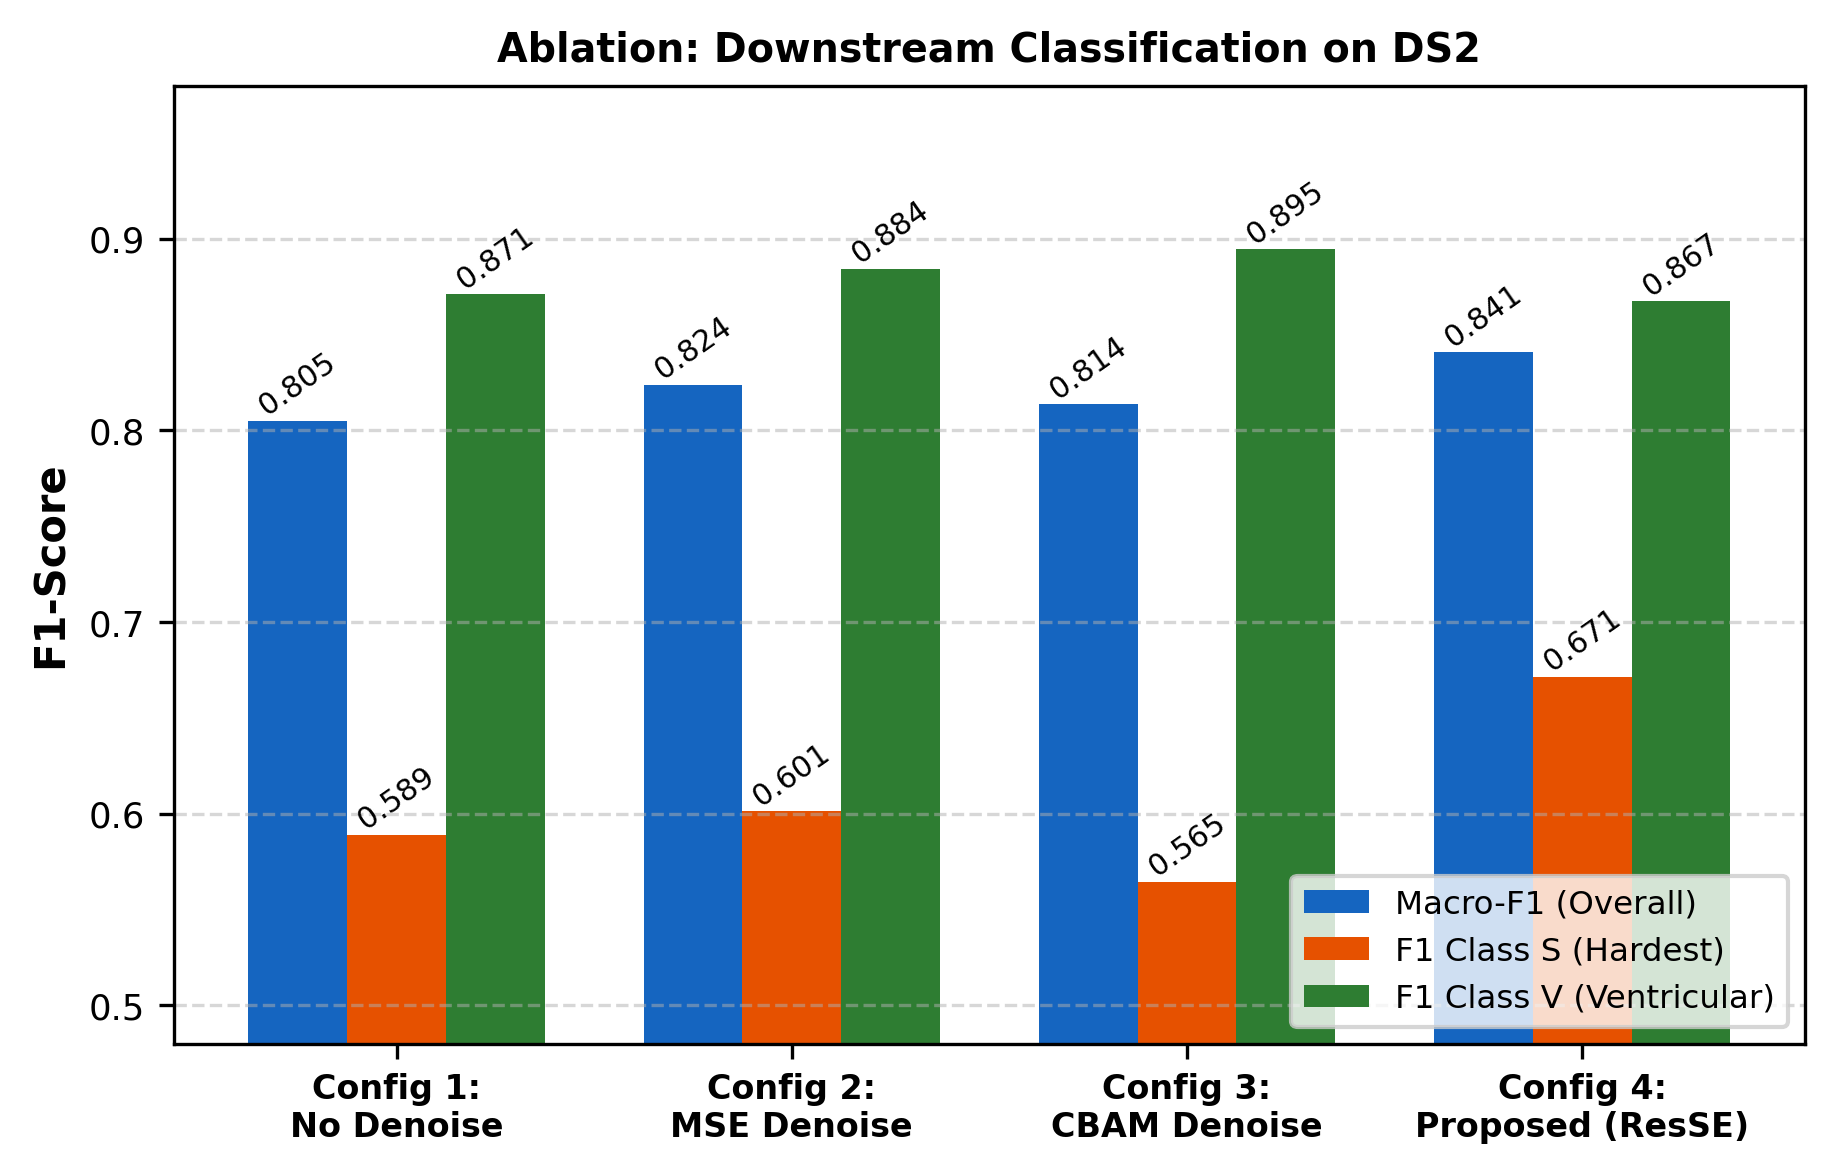
\includegraphics[width=\columnwidth]{Fig/fig6_ablation_f1_comparison.png}
\caption{Ablation study comparing 4 pipeline configurations on DS2 downstream classification F1-scores.}
\label{fig:ablation_f1}
\end{figure}

\begin{table*}[!t]
\caption{Ablation Study: Influence of Upstream Denoising on Downstream Inter-Patient Classification (Macro-F1)}
\label{tab:ablation_study}
\centering
\resizebox{\textwidth}{!}{%
\begin{tabular}{@{}cllrrrr@{}}
\toprule
ID & Upstream Denoiser & Loss Objective & Classical Mean & Classical Ens. & Hybrid Mean & Hybrid Ens. \\
\midrule
1 & Raw Contaminated & None & 0.7939 & 0.8050 & \best{0.8059} & 0.8102 \\
2 & \HSL{} (SE1D) & MSE Loss & 0.7857 & \second{0.8238} & 0.7642 & 0.8036 \\
3 & \HSL{} (CBAM1D) & Mixed Loss & 0.7894 & 0.8136 & 0.7877 & \second{0.8154} \\
4 & \textbf{\HSL{} (ResSE)} & \textbf{Mixed Loss} & \best{0.8092} & \best{0.8407} & \second{0.7897} & \best{0.8176} \\
\bottomrule
\end{tabular}%
}
\end{table*}

\subsection{Latent Feature Space Visualizations via UMAP}
To investigate how denoising and feature fusion facilitate clinical discrimination, Uniform Manifold Approximation and Projection (UMAP) was performed on latent representations. 

\begin{figure*}[!t]
\centering
\begin{minipage}{0.48\textwidth}
  \centering
  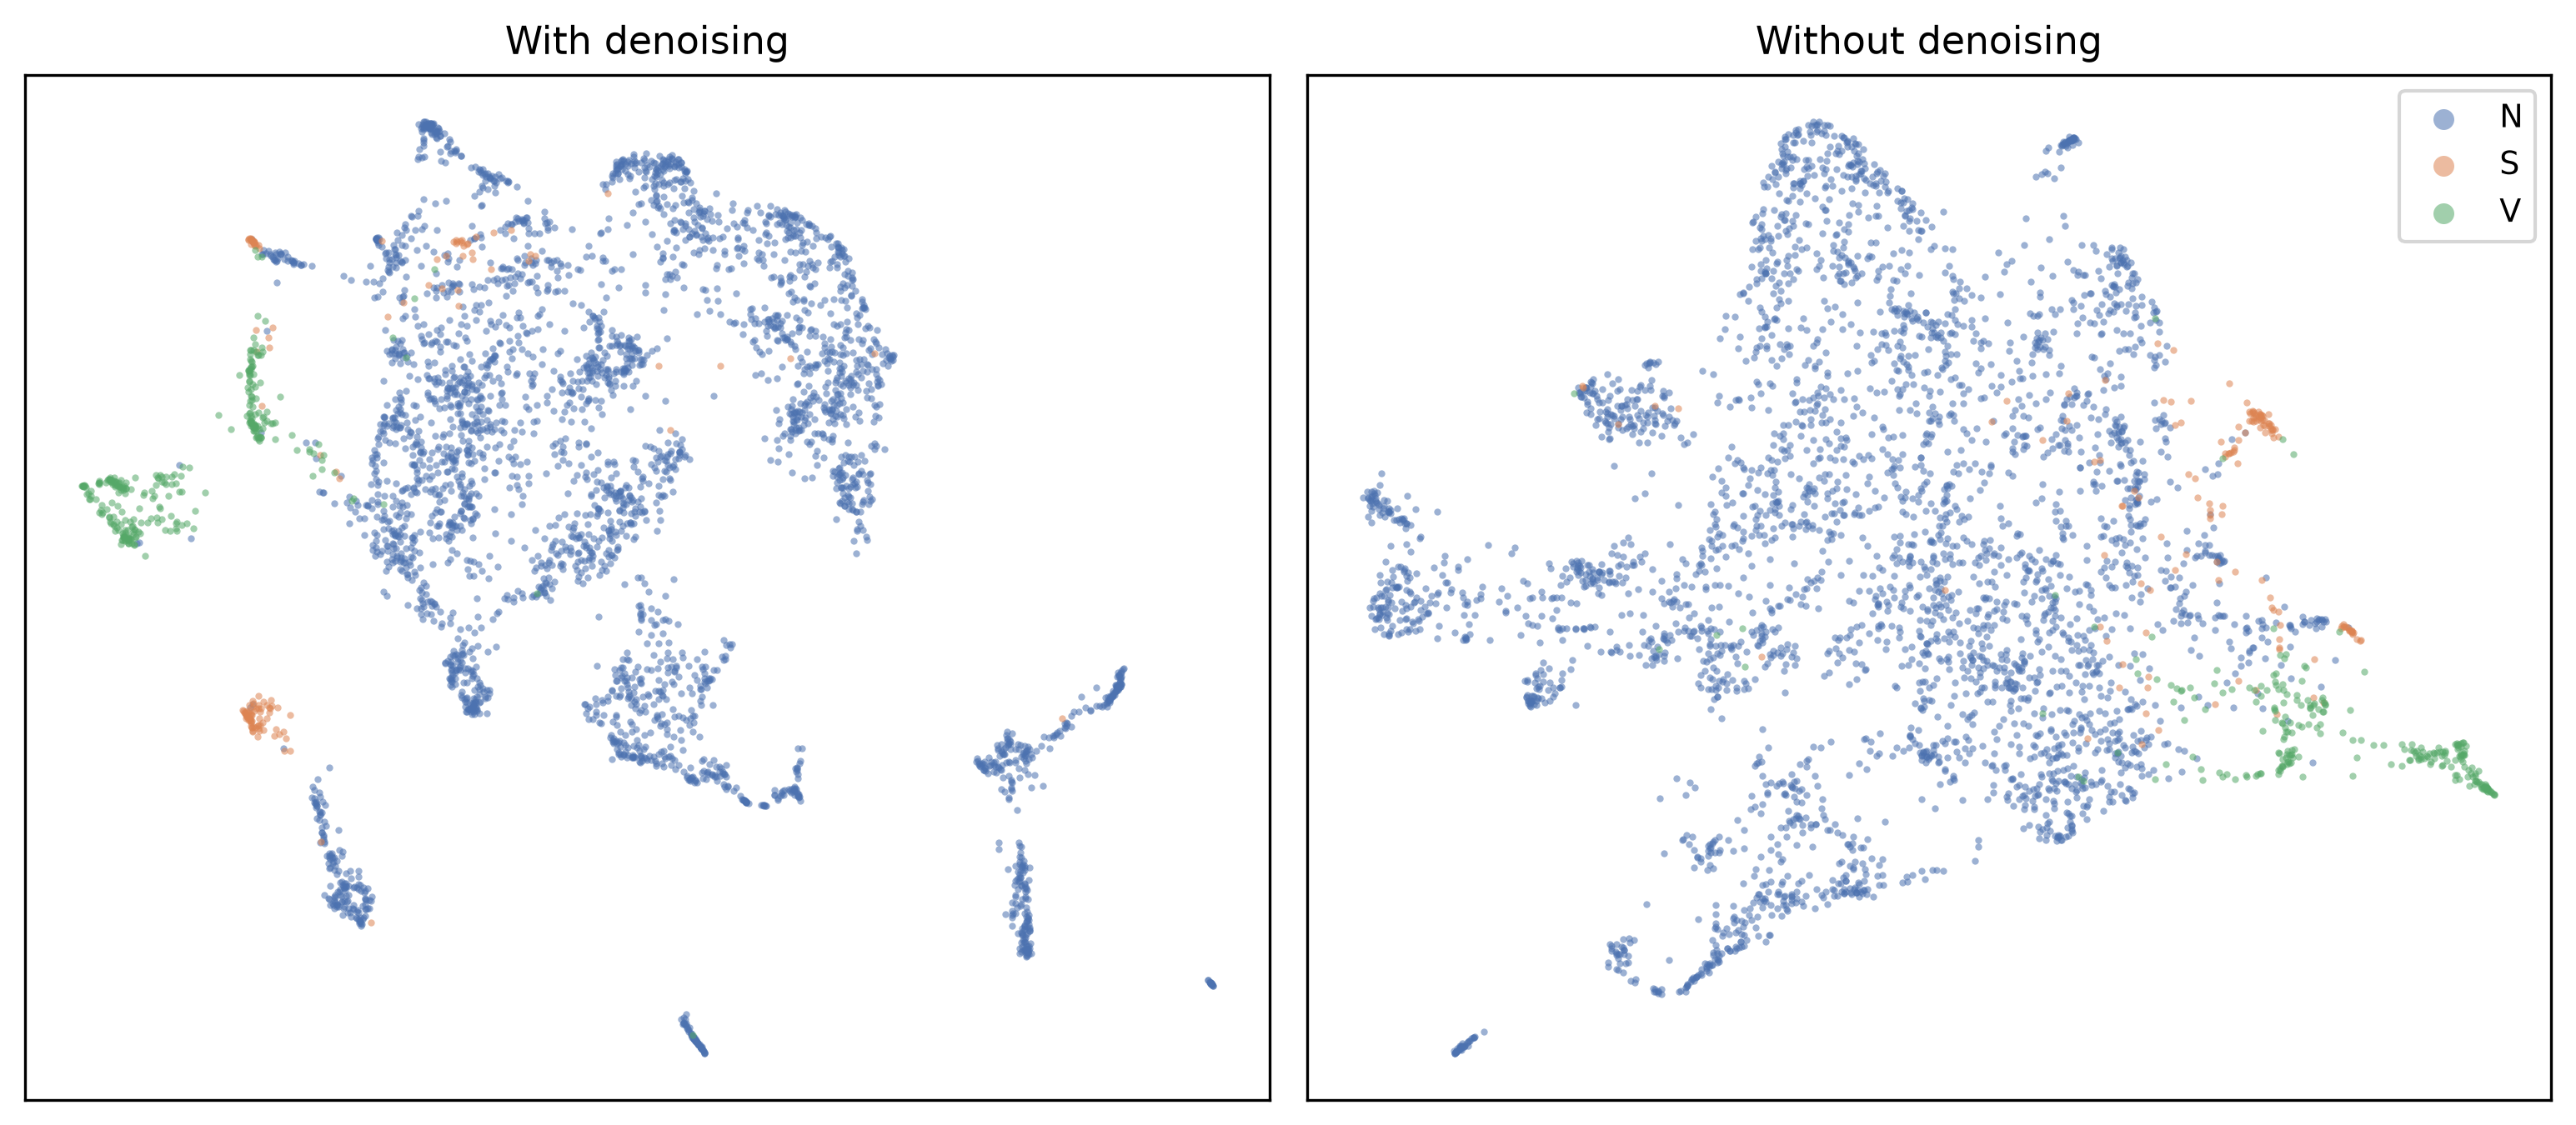
\includegraphics[width=\linewidth]{Fig/umap_denoise.png}
  \centerline{\footnotesize (a) Latent feature manifold before and after \HSL{} denoising.}
\end{minipage}\hfill
\begin{minipage}{0.48\textwidth}
  \centering
  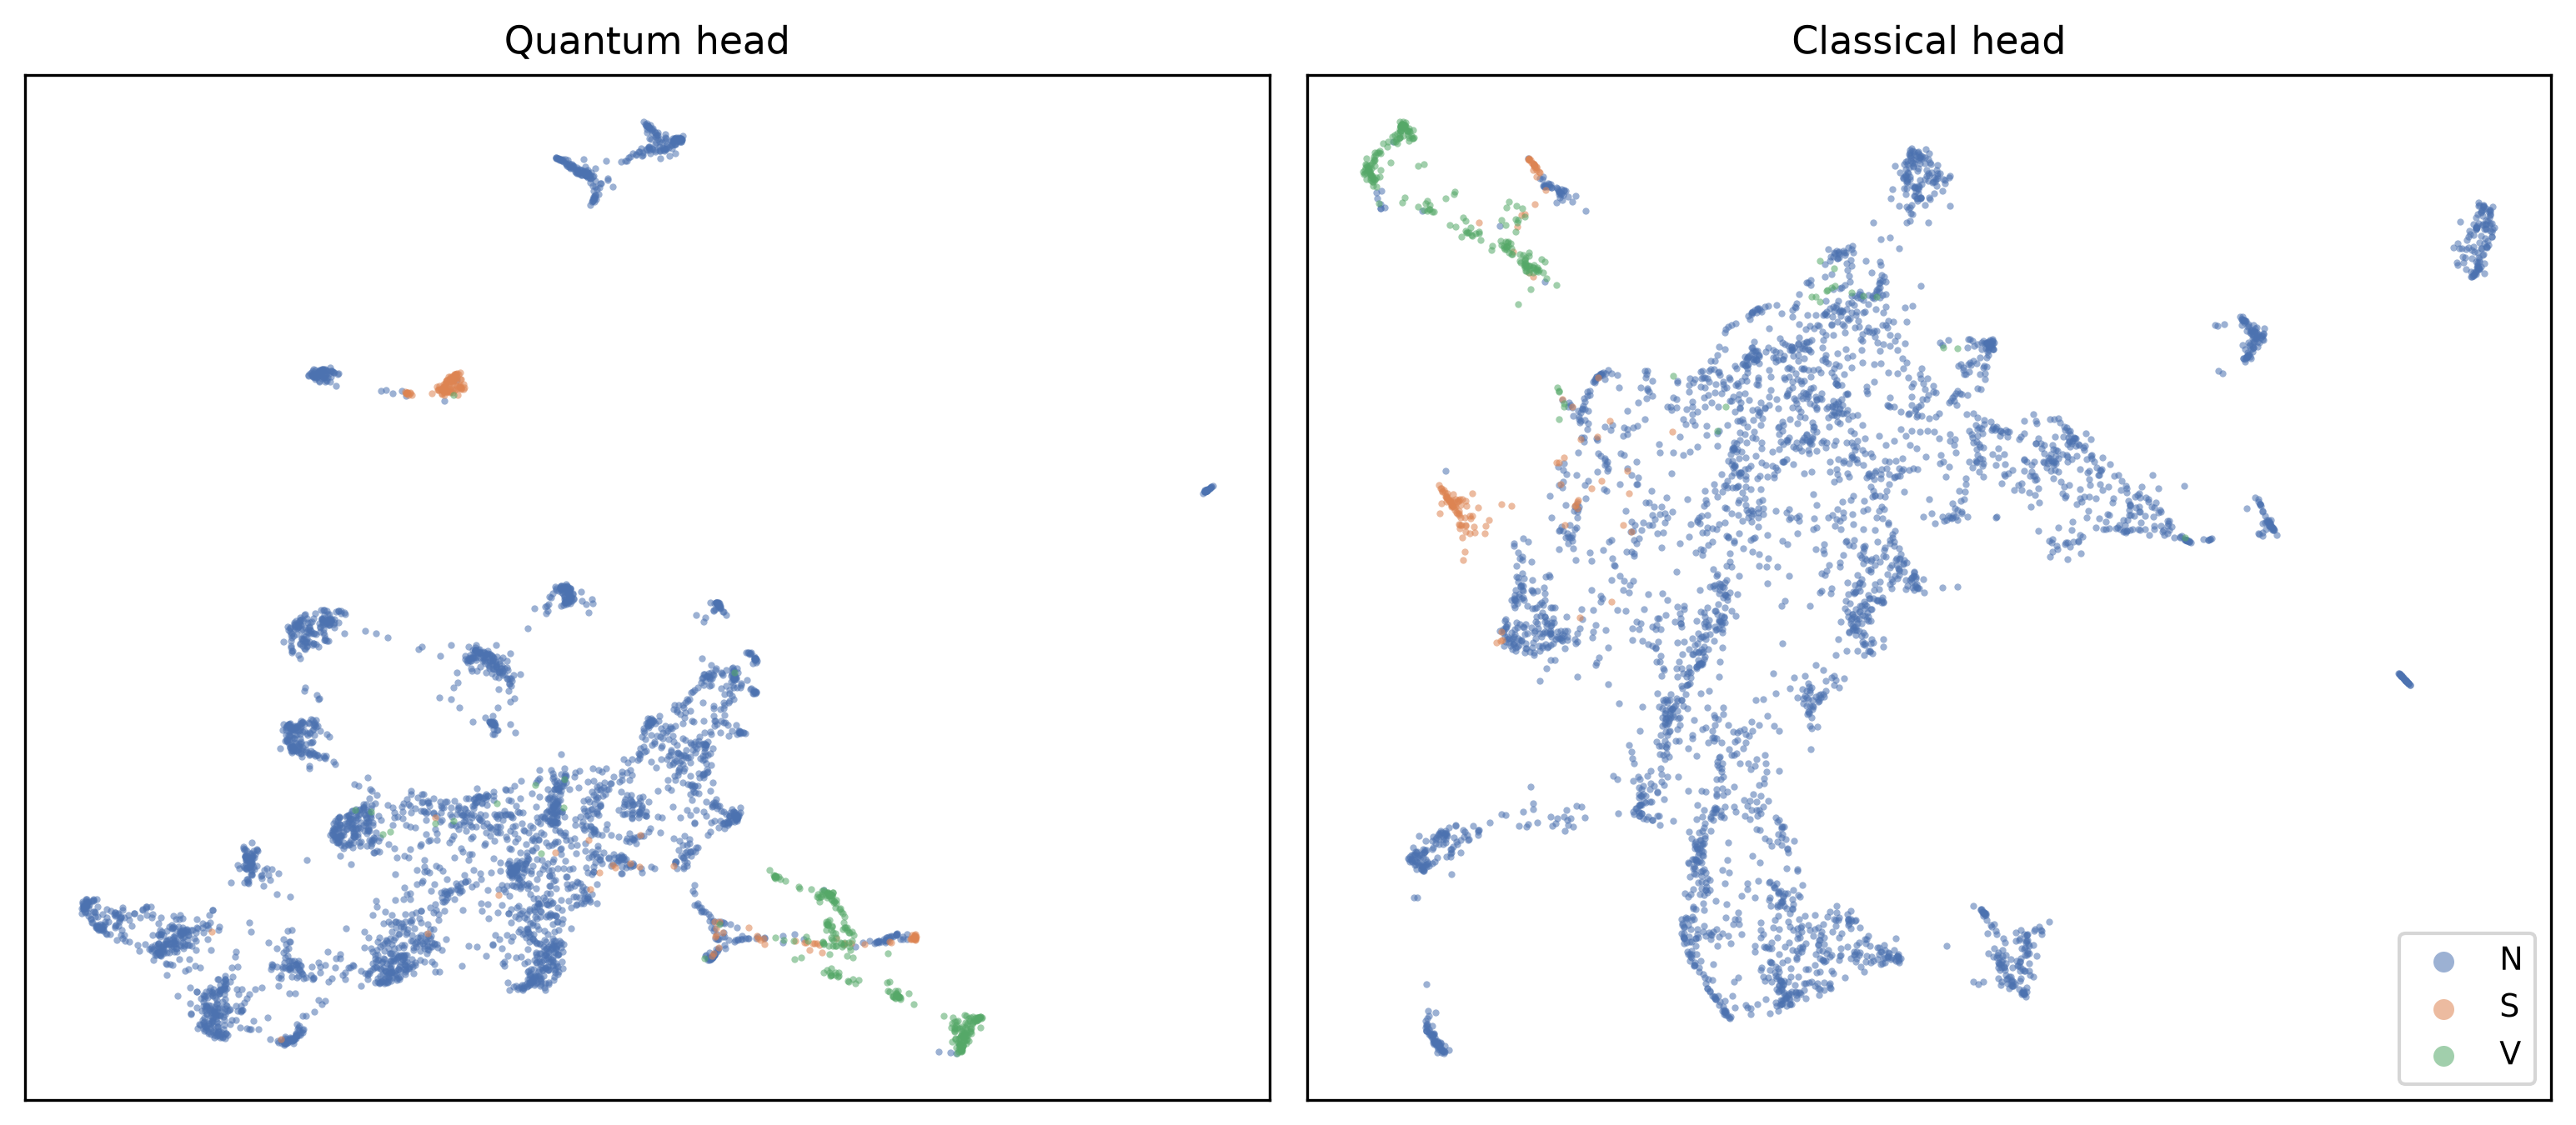
\includegraphics[width=\linewidth]{Fig/umap_head.png}
  \centerline{\footnotesize (b) 2D UMAP projection of the 160D joint latent space for N, S, and V classes.}
\end{minipage}
\caption{UMAP latent space visualizations: (a) noise suppression trajectory, and (b) diagnostic arrhythmia class separation.}
\label{fig:umap_combined}
\end{figure*}

Fig.~\ref{fig:umap_combined}(a) demonstrates that before denoising, severe noise sources collapse the feature manifold into entangled, overlapping distributions. After \HSL{} filtering, clear, separated manifold trajectories emerge, corresponding to true cardiac potentials. Fig.~\ref{fig:umap_combined}(b) visualizes the 160D joint latent space produced by \RRN. Despite the high morphological similarity between normal beats and supraventricular ectopics, the combination of 1D ResNet morphological features with the 6D RR contextual pathway achieves clean cluster separation across N, S, and V classes, corroborating our quantitative diagnostic results.
